\documentclass[11pt,a4paper,oneside,extrafontsizes]{memoir}

\renewcommand*{\baselinestretch}{1.04}
\isopage
\setlrmargins{*}{*}{1}
\checkandfixthelayout
%\documentclass[11pt,a4paper,twoside,openright,extrafontsizes]{memoir}

\renewcommand*{\baselinestretch}{1.04}
\isopage
\checkandfixthelayout
\usepackage{include/thesis}

\newcommand*{\bme}{Budapest University of Technology and Economics}
\newcommand*{\vik}{Faculty of Electrical Engineering and Informatics}

\newcommand*{\bmemit}{Department of Measurement and Information Systems}

\newcommand*{\vikdoctype}{Master's Thesis}
\newcommand*{\viktdkyear}{2016}

\newcommand*{\authors}{Author}
\newcommand*{\advisors}{Supervisors}

\newcommand*{\authori}{Dániel Stein}

\newcommand*{\advisori}{Gábor Szárnyas}
\newcommand*{\advisorii}{Ádám Lippai}
\newcommand*{\advisoriii}{Dávid Honfi}

\title{Graph-Based Source Code Analysis of JavaScript Repositories}
%\newcommand*{\titlepagetitle}{Graph-Based\\Source Code Analysis\\of JavaScript Repositories}
\newcommand*{\titlepagetitle}{Graph-Based\\Source Code Analysis\\of Dynamically Typed Languages}
\author{\authori}

\hypersetup{
  pdftitle={\thetitle},
  pdfauthor={\theauthor, \advisors: \advisori, \advisorii, \advisoriii}
  bookmarks=true,            % show bookmarks bar?
  unicode=true,              % non-Latin characters in Acrobat's bookmarks
  pdfnewwindow=true,         % links in new window
  colorlinks=true,           % false: boxed links; true: colored links
  linkcolor=black,           % color of internal links
  citecolor=black,           % color of links to bibliography
  filecolor=black,           % color of file links
  urlcolor=black             % color of external links
}


\usepackage{marginnote}
\usepackage{epigraph}
\newcommand{\code}[1]{{\upshape\ttfamily\small\indent #1}}

\bibliography{bibliography}

\begin{document}

\frontmatter{}

\thispagestyle{empty}

\begin{tikzpicture}[overlay,remember picture]
  \node at (current page.center) [yshift=1cm] {%
    \begin{minipage}{\textwidth}

      \centering

      
\includegraphics[width=7cm]{include/figures/bme_logo}
      \vspace{0.3cm}

      \bme \\
      \vik \\
      \bmemit \\
      \vspace{3.5cm}

      {\Huge\sffamily\bfseries \titlepagetitle \par}
      \vspace{1cm}

      {\large \vikdoctype \par}
      \vspace{2cm}

      {\Large
        \authors: \\ \vspace{0.3cm}
        \authori

        \vspace{1cm}
        \advisors: \\ \vspace{0.3cm}
        \advisori \\
        \advisorii\par}

      \vspace{1.5cm}
      {\large \viktdkyear.\par}

    \end{minipage}};
\end{tikzpicture}

\cleardoublepage

\tableofcontents

\selectenglish{}
{
\selecthungarian{}
\begin{center}
\large
\textbf{HALLGATÓI NYILATKOZAT}\\
\end{center}

Alulírott \emph{Stein Dániel}, szigorló hallgató kijelentem, hogy ezt a diplomatervet meg nem engedett segítség nélkül, saját magam készítettem, csak a megadott forrásokat (szakirodalom, eszközök stb.) használtam fel. Minden olyan részt, melyet szó szerint, vagy azonos értelemben, de átfogalmazva más forrásból átvettem, egyértelműen, a forrás megadásával megjelöltem.

Hozzájárulok, hogy a jelen munkám alapadatait (szerző(k), cím, angol és magyar nyelvű tartalmi kivonat, készítés éve, konzulens(ek) neve) a BME VIK nyilvánosan hozzáférhető elektronikus formában, a munka teljes szövegét pedig az egyetem belső hálózatán keresztül (vagy autentikált felhasználók számára) közzétegye. Kijelentem, hogy a benyújtott munka és annak elektronikus verziója megegyezik. Dékáni engedéllyel titkosított diplomatervek esetén a dolgozat szövege csak 3 év eltelte után válik hozzáférhetővé.

\begin{flushleft}
\vspace*{1cm}
Budapest, \today
\end{flushleft}

\begin{flushright}
 \vspace*{1cm}
 \makebox[7cm]{\rule{6cm}{.4pt}}\\
 \makebox[7cm]{\emph{Stein Dániel}}\\
 \makebox[7cm]{hallgató}
\end{flushright}
\thispagestyle{empty}

\vfill
\clearpage
\thispagestyle{empty} % an empty page

}

\begin{otherlanguage}{magyar}

  \paragraph*{Kivonat}
  \phantomsection
  \addcontentsline{toc}{chapter}{Kivonat}
  \thispagestyle{plain}
  {
  \selecthungarian

  Egyre több, egyre inkább komplex szoftver vesz körül minket, sok esetben ezek akár részét képezhetik kritikus rendszereknek is. Az ilyen rendszerek fő jellemzője, hogy a legapróbb hibáik is komoly következményekkel járhatnak. A forráskód statikus analízise egy, a kritikus szoftverrendszereknél általánosan elfogadott megközelítés, amely a hibák mihamarabbi megtalálását célozza meg.  A statikus analízis már a fejlesztési folyamat korai szakaszaiban is alkalmazható, mivel nincs szükség a kód fordítására és futtatására az ellenőrzés véghezviteléhez. A megközelítést számos eszköz megvalósítja, amelyek képesek visszajelzést adni a potenciális hibahelyeken túl arról is, hogy a forráskód megfelel-e a kódolási szabályoknak és követelményeknek.

  Habár több statikus analízis eszköz is elérhető generikus nyelvek elemzéséhez, és ezek többsége beépíthető a folytonos integráció folyamatába is, JavaScript esetén ez nem mondható el annak dinamikus volta végett. A dinamikus nyelvek sajátosságai miatt csak pár eszköz érhető el JavaScript forráskódok kódtárszintű statikus analíziséhez, illetve az eddig ismert ilyen eszközök nem nyújtanak egyszerre megoldást alaki ellenőrzésre, futási utak meghatározására és folytonos integrációba történő integrációra.
  
  Jelen dolgozatomban egy olyan, a folytonos integráció kiegészítésére képes keretrendszert tervezek, valósítok meg és értékelek, amely képes nagyméretű és gyakran változó JavaScript forráskódtárak konfigurálható statikus analízisére. A keretrendszer alapjául szolgáló újszerű megközelítésnek köszönhetően az eddig megszokott megoldások helyett a felhasználók egyszerűbb módon fejezhetik ki az ellenőrzésre szánt követelményeket és képesek a több forráskódon átívelő követelményeket hatékonyabban elemezni.

  }

\end{otherlanguage}

\cleardoublepage

\paragraph*{Abstract}
\phantomsection
\addcontentsline{toc}{chapter}{Abstract}
\thispagestyle{plain}

We are surrounded by more and more complex software that operate in mission-critical systems. Even small errors in these software can lead to consequences ranging from unpleasant to expensive. A proven approach for detecting mistakes early in the development cycle is static analysis of the source code. Static analysis tools report whether the software conforms to the coding rules and requirements without executing the code itself.

While multiple static analysis tools exist for general purpose programming languages and these are generally part of the continuous integration systems, this is not the case with JavaScript. Because of the untyped nature of this dynamic language there are only a few tools that perform static analysis on JavaScript code repositories on a global level.

In this report I design, implement and evaluate a framework aiming to extend the continuous integration workflow of large JavaScript repositories with various static analysis tools and techniques.

\clearpage

\newcounter{savepage}
\setcounter{savepage}{\arabic{page}}

\mainmatter{}

\chapter{Introduction}
\label{chap:introduction}

\section{Context}

Quality control plays an important role in large-scale software development. The number of coding errors are noticeably increasing with the number of contributors. The more developers work together on developing a software, the more versatile their coding styles and conventions are.

To ensure the quality of the source code, thus the software itself, and at the same time help developers with their tasks, the need arises for a solution continuously reviewing the code, searching for mistakes, and enforcing conventions.

\begin{figure}[!ht]
	\centering
	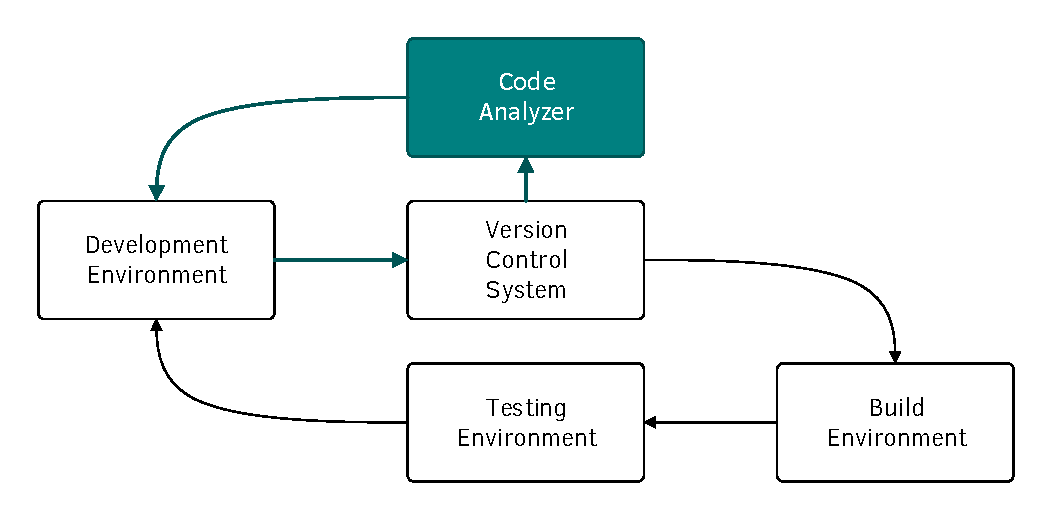
\includegraphics[height=6cm]{CI-workflow}
	\caption{Continuous Integration workflow extended with Static Analysis.}
	\label{fig:CI-workflow}
\end{figure}

Version control systems (VCS) and continuous integration (CI)~\cite{CI} are widely used tools of the modern software developers. \Cref{fig:CI-workflow} shows an extended version of the generally used continuous integration workflow.
The basic workflow consists of the following steps. The developer makes modifications to the codebase using their \textit{Development Environment}. The modifications are committed into a \textit{Version Control System}, and this commit triggers the \textit{Build Environment} to build the project. The \textit{Testing Environment} can then perform runtime tests on latest build of the project. After this process, the results --- build and test logs --- are presented to the developer.

These logs help the developers discover bugs and failures before the software is released for manual testing or production purposes. Producing this information and making sure the software is working as intended often and early in the development workflow is vital for agile development.

A proven method of enhancing software quality is utilizing static program analysis techniques supplementing the basic CI workflow. During this method, the code is analyzed without executing the application. In practice, this method is able to reveal problems that are undetectable with testing and thus is able to aid the developer in creating higher quality software.


\section{Problem Statement}

Static analysis methods verifying that the code is compliant with coding conventions are often time consuming and resource intensive in practice. The size of the codebase may require a scalable solution, especially for continuous integration purposes, since the entire verification process needs to be carried out on the whole codebase once it is (partially) modified.

A temporary solution to tackle this problem is to process the changes in batches. To save resources, static analysis runs are carried out for a joined group of changes, rather than for every individual commit.

In an ideal situation, even before committing the changes, the developers receive feedback about the problems their modifications would imply.


\section{Objectives and Contributions}

My main objective is to provide a solution for reducing the time required for global, codebase-level reevaluation of static analysis after a change occurs.

I aim to create a framework that transforms the whole source code repository into a graph representation and maintains it subsequently. It should perform code convention compliance checks, execute built-in static analysis tests and be extended with arbitrary tests by the user.

Incremental processing is one of the possible solutions for speeding up static analysis. Thus it should be able to process a subset of the repository, e.g. only the modifications introduced by the latest commit, then integrate the changes into the maintained representation. This way the system can process the modifications in a commit incrementally. After the initial query evaluation and report generation, consecutive runs can be executed significantly more efficiently.

The framework relies on two substantial technologies --- a source code parser and an adequate database solution --- and provides interfaces making integration possible with external tools, such as version control systems and integrated developer environments.


\section{Structure of the Thesis}

This thesis is structured as follows.
\Cref{chap:preliminaries} introduces the previously mentioned background technologies required and selected to build an incremental static analyzer.
\Cref{chap:background-and-related-work} details the various approaches and related researches.
\Cref{chap:overview-of-the-approach} shows the overview of my approach and gives detailed view of the main components of its architecture.
\Cref{chap:elaboration-of-the-workflow} presents the implementation of the framework, and discusses the steps of the analysis.
\Cref{chap:evaluation-of-the-prototype} demonstrates and evaluates the performance of the framework.
\Cref{chap:future-vision} reveals future vision ideas and possibilities.
\Cref{chap:conclusions} concludes the thesis.

% !TEX root = ../main.tex
\chapter{Background and Related Work}
\label{chap:background-and-related-work}

In this chapter I introduce the conceptual foundations and used technologies of my work. Here I discuss the building blocks required to create a static analyzer framework for JavaScript. I also enumerate a subset of similar systems and discuss related work.

\section{JavaScript}
\subsection{Overview of the Last Few Years}
\subsection{The Future of JavaScript}

\section{Modeling}
Modeling is a versatile concept, the word itself may refer to various topics. In the context of this thesis, by models I primarily mean data models. A data model ---or sometimes called domain model--- organizes the data elements, how they relate to each other and what actions one can perform on them.

\subsection{Metamodels and Instance Models}
Metamodeling is a methodology for the definition of modeling languages. A metamodel specifies the abstract syntax (structure) of a modeling language.~\cite{scm}

The metamodel contains the main concepts and relations of the domain specific language (DSL) and defines the possible structure of the instance models. To enrich the expressive power of the language, attributes are added to the concepts. By doing this, the language can be extended with predefined domains of data types (like integers, strings) that are supported by the metamodeling language. Additionally, some structural constraints might be specified with the elements like multiplicity.

Models describing a particular problem in the domain, called instance models, are defined using the elements of the metamodel.

\section{Static Analysis}
\textquote[\cite{wichmann_industrial_1995}]{The idea  that  computer  software  should be used to analyse source programs rather than compile them, has a history of at least 25 years.}

We use program analysis to discover facts about it. Two basic automated analysis methods exist for source code analysis. When the source code is read and analyzed without evaluating the statements or executing it, we talk about static analysis. Analysis with statement evaluation or execution is known as dynamic analysis.

% > The term is usually applied to the analysis performed by an automated tool, with human analysis being called program understanding, program comprehension, or code review. Software inspections and Software walkthroughs are also used in the latter case.
% https://en.wikipedia.org/wiki/Static_program_analysis

While JavaScript may not be, high-level language source codes are at least audited by the compiler. Thus the aim of a specific analysis should be discovering unwanted traits of the source in ways a generic compiler could not do, resulting in better code quality. These treats, \emph{bugs} are usually perceptable while running the code. Another way to locate these bugs is to write and run tests, but it may not worth it, if there is a better solution.
% \cite[][72]{wichmann_industrial_1995}

% > Static analysis bug-finding tools have evolved over the last several decades from basic syntactic checkers to those that find deep bugs by reasoning about the semantics of code. The goal of the Clang Static Analyzer is to provide a industrial-quality static analysis framework for analyzing C, C++, and Objective-C programs that is freely available, extensible, and has a high quality of implementation.
% http://clang-analyzer.llvm.org/


\subsection{Use Cases}
The level of abstraction of the static analysis tools varies. Formatters make sure that the source code complies with the style guide. Linters check for stylistic and programming errors and warn at suspicious programming constructs. Formal verification, on the other hand, utilizes formal mathematical methods to prove or refute statements about the source code and its behavior.

For dynamic languages, it can be used for even more\footnote{Non-exhaustive list}: finding previously undefined property reads, invoke of non-functional variables~\cite{jensen_type_2009} or dead code.

\subsection{Advantages and Disadvantages}

Since static analysis tools deliberately do not evaluate the source code, there are fundamental limitations to what problems they can discover. I consider the following advantages and disadvantages important.


\subsubsection{Advantages}
\paragraph{Input Data Is a By-Product of Compilers}

\paragraph{No Need for Execution}
\begin{itemize}
  \item no need for run environment
  \item no need for mocking, emulating
\end{itemize}

\subsubsection{Disadvantages}
\paragraph{Speed} Static analysis trades CPU time and memory for better code quality. By design it may be multiple magnitudes slower than compilation, but its speed depends not only on the underlying data structure and algorithms, but the level of analysis too.
%  > Slower than Compilation
%
%  > Operationally, using static analysis to automatically find deep program bugs is about trading CPU time for the hardening of code. Because of the deep analysis performed by state-of-the-art static analysis tools, static analysis can be much slower than compilation.
%
%  > While the Clang Static Analyzer is being designed to be as fast and light-weight as possible, please do not expect it to be as fast as compiling a program (even with optimizations enabled). Some of the algorithms needed to find bugs require in the worst case exponential time.

Although, with a given limitation of granularity, in case of a source code modification, previous results can be reused. There is a possibility that only the modified ---and other affected--- parts need to be analyzed again. The incremental approach of static analysis may speed up the process by orders of magnitude~\cite{stein-daniel-bsc}.

\paragraph{False Positives} Static analysis can not prove the soundness of a source code. It rather warn in case there is a possibility of a problem. Thus static analysis tools can introduce false positive warnings and flag code parts even if they behave correcly.

To reduce the number of false positive warnings, one usually introduces more precise, specified rules and more thorough analysis.

%  > False Positives
%
%  > Static analysis is not perfect. It can falsely flag bugs in a program where the code behaves correctly. Because some code checks require more analysis precision than others, the frequency of false positives can vary widely between different checks. Our long-term goal is to have the analyzer have a low false positive rate for most code on all checks.
%
%  % http://clang-analyzer.llvm.org/

\subsection{Typed JavaScript Derivations}

\subsection{Type Inference}

Type inference refers to the deduction of the data types of expressions, statements during static analysis.

> Type inference refers to the automatic deduction of the data type of an expression in a programming language. If some, but not all, type annotations are already present it is referred to as type reconstruction[citation needed]. The reverse operation of type inference is called type erasure.

> It is a feature present in some strongly statically typed languages. It is often characteristic of functional programming languages in general. Some languages that include type inference are Nim, ML, OCaml, F\#, Haskell, Scala, Go, D, Clean, Opa, Rust, Swift, Visual Basic (starting with version 9.0), C\# (starting with version 3.0) and C++11. The ability to infer types automatically makes many programming tasks easier, leaving the programmer free to omit type annotations while still permitting type checking.

% https://en.wikipedia.org/wiki/Type_inference

\subsubsection{Flow}
> Flow, a new open-source static type checker for JavaScript. Flow adds static typing to JavaScript to improve developer productivity and code quality. In particular, static typing offers benefits like early error checking, which helps you avoid certain kinds of runtime failures, and code intelligence, which aids code maintenance, navigation, transformation, and optimization.

% https://code.facebook.com/posts/1505962329687926/flow-a-new-static-type-checker-for-javascript/

> Flow can infer the type of most things within a file, so you don't always have to annotate every function and variable to get typechecking to work. However, even if Flow can infer a type, you can still add annotations to be explicit. The only time that Flow strictly requires an annotation is when a variable/function/class is exported from a module (defined in one file and used in another).
>
> In our final example, 05\_DynamicCode, we haven't annotated the function, but we are passing in two different types of arguments:
>
> In this case, Flow detects that the second time the function is called (with a number), the length property will fail:
>
> Flow is smart enough to detect that this conditional check is sufficient to avoid any potential failures at run time, and will give you a clean bill of health.

% http://flowtype.org/docs/five-simple-examples.html#2-adding-type-annotations

> Since types are not part of the JavaScript specification, we need to strip them out before sending the file to the user.

% http://flowtype.org/docs/running.html#using-the-offline-transform-tool

> Making previously-untyped code typecheck with Flow may take some time and work - and sometimes it may not be worth the effort in the short term. Flow supports interface files so you can use libraries in a typed way without having to run Flow on them at all. If your project just depends on third party libraries, check out our guide on using Flow with external dependencies and consider using an interface file for the libraries.
>
>Why is typechecking existing code so hard? Libraries not written with types in mind often contain complex, highly dynamic code that confuses analyzers such as Flow. The code may also have been written in a style that Flow deliberately chooses not to support in order to give the programmer more help. Some typical examples are:
>
>    Operations on primitive values: While JavaScript allows operations such as true + 3, Flow considers it a type error. This is by design, and is done to provide the programmer with more safety. While that's easily avoided for new code, it can sometimes be a lot of effort to eliminate such patterns from existing code.
>    Nullability: Flow protects you against accessing properties on null by tracking null or undefined values throughout the program. In large existing codebases, though, this can require inserting some extra null checks in places where a value appears like it may be null, but actually isn't at runtime.
>
> It is typically a much larger effort, and requires much more programmer annotation, to get such code to typecheck. On the other hand, if you own a library and would like to benefit from Flow typechecking within the library itself, this guide is for you.

% http://flowtype.org/docs/existing.html

> When you start Flow, it performs an initial analysis of all the files in your codebase and stores the results in a persistent server. When you save a file, Flow incrementally rechecks the changes in the background.
>
> Both the initial analysis and recheck are heavily optimized for performance, which preserves the fast feedback of developing plain JavaScript.
>
> Flow uses control flow analysis to deeply understand your code to find errors that other type systems can't. Flow is designed to find errors and we take soundness seriously.
>
> For example, Flow tracks null values which may propagate unintentionally through code and eventually cause a runtime error. Flow's path sensitive analysis can uncover bugs like this, even through layers of indirection in the program's control flow

% http://flowtype.org/docs/about-flow.html#_

> Facebook loves JavaScript; it’s fast, it’s expressive, and it runs everywhere, which makes it a great language for building products. At the same time, the lack of static typing often slows developers down. Bugs are hard to find (e.g., crashes are often far away from the root cause), and code maintenance is a nightmare (e.g., refactoring is risky without complete knowledge of dependencies). Flow improves speed and efficiency so developers can be more productive while using JavaScript.

> But layering a static type system onto JavaScript is not trivial. JavaScript’s building blocks are extremely expressive, and simple type systems do not suffice to precisely model their semantics. To seamlessly work with several common JavaScript idioms, Flow employs the kind of data-flow and control-flow analysis that compilers typically perform to extract semantic information from code. It then uses this information for type inference, building on advanced techniques in type theory. Of course, designing a powerful static analysis is not sufficient — JavaScript codebases can be huge, so type checking has to be blazing fast as not to disrupt the developer’s edit-run cycle. Flow performs its analysis modularly, guided by types at module boundaries. This enables an aggressively parallel and incremental type checking architecture, similar to Hack. This allows type checking to appear instantaneous, even on millions of lines of code.
>
> Flow’s type checking is opt-in — you do not need to type check all your code at once. However, underlying the design of Flow is the assumption that most JavaScript code is implicitly statically typed; even though types may not appear anywhere in the code, they are in the developer’s mind as a way to reason about the correctness of the code. Flow infers those types automatically wherever possible, which means that it can find type errors without needing any changes to the code at all. On the other hand, some JavaScript code, especially frameworks, make heavy use of reflection that is often hard to reason about statically. For such inherently dynamic code, type checking would be too imprecise, so Flow provides a simple way to explicitly trust such code and move on. This design is validated by our huge JavaScript codebase at Facebook: Most of our code falls in the implicitly statically typed category, where developers can check their code for type errors without having to explicitly annotate that code with types.

% https://code.facebook.com/posts/1505962329687926/flow-a-new-static-type-checker-for-javascript/

\begin{itemize}
\item \url{http://flowtype.org/}
\item \url{https://github.com/facebook/flow}
\item \url{https://code.facebook.com/posts/1505962329687926/flow-a-new-static-type-checker-for-javascript/}
\end{itemize}


\subsubsection{TAJS}
\textquote[\cite{tajs-git}]{TAJS is a dataflow analysis for JavaScript that infers type information and call graphs. The current version of the analysis contains a model of ECMAScript 3rd edition, including the standard library, and a partial model of the HTML DOM and browser API.}

TAJS initially (in 2009) tried to warn programmers for the following problematic cases. This enumeration follows~\cite{jensen_type_2009}.

\begin{enumerate}
  \item invoking a non-function value as a function
  \item reading an absent variable
  \item accessing a property of \code{null} or \code{undefined}
  \item reading an absent property of an object
  \item writing to variables or object properties that are never read
  \item implicitly converting a primitive value to an object
  \item implicitly converting \code{undefined} to a number
  \item calling a function object both as a function and as a constructor or passing function parameters with varying types
  \item calling a built-in function with an invalid number of parameters orwith a parameter of an unexpected type
\end{enumerate}

\begin{itemize}
 \item \url{http://www.brics.dk/TAJS/}
 \item \url{https://github.com/cs-au-dk/TAJS}
 \item \url{http://www.srl.inf.ethz.ch/workshop2014/eth-moeller.pdf}
\end{itemize}

\subsubsection{Tern}
\begin{itemize}
 \item \url{http://marijnhaverbeke.nl/blog/tern.html}
 \item \url{http://ternjs.net/doc/manual.html#infer}
 \item \url{http://ternjs.net/doc/manual.html#typedef}
 \item \url{https://github.com/angelozerr/tern.java}
 \item \url{https://github.com/ternjs/tern/blob/master/lib/infer.js}
\end{itemize}

\subsubsection{JSNice -- Programming Tools with Big Data and Conditional Random Fields (ETHZ)}
\begin{itemize}
 \item \url{http://www.srl.inf.ethz.ch/jsnice.php}
 \item \url{http://www.srl.inf.ethz.ch/papers/jsnice15.pdf}
 \item \url{http://www.jsnice.org/}
 \item \url{https://github.com/eth-srl/Nice2Predict}
\end{itemize}

\subsubsection{Mozilla DoctorJS}
\begin{itemize}
\item \url{http://rfrn.org/~shu/drafts/ti.pdf} (2012)
\item \url{https://wiki.mozilla.org/TypeInference}
\item \url{https://github.com/dimvar/doctorjs}
\item \url{https://github.com/mozilla/doctorjs}
\end{itemize}

\subsubsection{JS0 -- PhD (2006) @ University of London}
\begin{itemize}
 \item \url{http://dev.pubs.doc.ic.ac.uk/chrisandersonphd/chrisandersonphd.pdf}
\end{itemize}

\subsubsection{Infernu}
\begin{itemize}
 \item \url{https://github.com/sinelaw/infernu}
\end{itemize}

\subsubsection{University of California}
\begin{itemize}
 \item \url{https://www.cs.ucsb.edu/~benh/research/papers/kashyap13type.pdf (2013)}
\end{itemize}


\section{Graph Databases}


\subsection{Adequate Database Solutions}
Since my thesis work is based on graph-based data handling, it is essential to use a technique that is suitable. In this case suitable is better described as being fast, flexible, versatile, easy to use and deploy. In this section I go over some of the most promising candidates and justify why I've chosen Neo4j as the foundation of my approach.

\subsubsection{Neo4j}
Neo4j is one of the most popular and most mature NoSQL graph databases developed by \emph{Neo Technology}. It's open-source, well-documented and steadily-developed. It's available in two editions: a free \emph{Community Edition} and a paid \emph{Enterprise Edition}.~\cite{neo4j}

\paragraph{Architecture}
Since Neo4j was written in Java (and Scala), it can be used to start a new project quick and easy. In respect of connection, it can be deployed two ways: in \emph{server mode} the database is started separately and listens for queries on its HTTP REST and Bolt interface; where in \emph{embedded mode} it runs in the same JVM as the only client application.

\paragraph{Data Model}
The graph model in Neo4j, \code{Neo4jGraph} is an implementation of the \emph{TinkerPop} graph computing framework's \emph{Blueprints} property graph data model. More precisely it is a labeled property graph, since the relations are labeled and the nodes can also hold multiple labels; the nodes and relations can both hold properties.

Unfortunately the relations are only binary, ternary (and n-ary $n>2$) relations can only be stored with an introduced indirection, a connection node connecting every node in the relation.

\paragraph{Sharding}
Although the \emph{Enterprise Edition} of Neo4j has a high availability solution and supports clustered replication and cache sharding, it does not support sharded data storage over a cluster of devices. This results in the advantage of low latency (clustering provides scale out capabilities for read), the ability to handle transactions and having ACID as the consistency model.~\cite{neo4j-product}

\paragraph{Query Language}
Neo4j provides two methods for data query out-of-the-box: an object-oriented native Java API for graph navigation and Cypher, a graph pattern description and query language with declarative and imperative traits. Additional interfaces may be loaded as a plugin, like the imperative Gremlin query interface~\cite{neo4j-gremlin-plugin}.

One of Cypher's best features is the readibility of its syntax. It provides an intuitive way to describe patterns of nodes and relations in the graph and also connections between subpatterns using bound identifiers for nodes and relations. Cypher also manages the indexes and constraints of the graph database. Negative application conditions (NAC) can be also expressed, describing the cases where the query should not return a match.

Other interesting and useful features of Cypher includes:
\begin{itemize}[topsep=0pt]
  \item Repetition bound (or unbound) transitive closure over an edge. The label of the edge can be also set to one label or a set of labels. Given sequence of labeled edges (with or without bound labels of nodes) can not be set on its own, but temporary edges can be utilized to emulate this behavior.
  \item Stored procedures are a very welcome new feature of the latest (as of May, 2016) Cypher and Neo4j version (v3.0). Procedures written in Java can be stored in the server as a plugin and called from the queries abolishing the need for manual logic-based calls in case it was not possible to formalize a query for it (ranging from duplicating a node (with parameters and labels) to infering the metamodel (from the nodes and relations already in the database)).
  \item Parametrized queries may be utilized for faster evaluation.
  \item List predicates evaluating predicates for all/any/none or single one nodes of the path.
  \item Iterating and unwinding a collection in the query
  \item Finding the shortest path
  \item Mathematical functions
  \item Query profiling
\end{itemize}

\textquote[\cite{neo4j-developer}]{Since October 2015 the openCypher project aims to provide an open grammar, language specification, technical compatibility kit and reference implementation of parser, planner and runtime for Cypher.}

\paragraph{Other Advantages and Disadvantages}
\begin{itemize}[topsep=0pt]
  \item[+] When Neo4j is deployed in server mode, besides the REST and Bolt interfaces, a web GUI is also available, where a read-evaluate-print loop (REPL) interface helps the user with interactive querying. The results are either shown in a table or an also interactive graph display, where the user can automatically add necessary nodes and relations from the database (without explicitly executing another query). It also supplies the user with information about the contents of the database, labels, indexes.
  \item[+] Graph Gists are interactive teaching tools allowing the visitor of the site to learn about various domains modeled in Neo4j and learn from the example queries.
\end{itemize}

\subsubsection{Titan}
\textquote[\cite{titan}]{Titan is a scalable graph database optimized for storing and querying graphs containing hundreds of billions of vertices and edges distributed across a multi-machine cluster. Titan is a transactional database that can support thousands of concurrent users executing complex graph traversals in real time.}

Titan was developed by \emph{Aurelius} until the company was aquired by \emph{DataStax} in 2015. DataStax has expressed its intentions to preserve the effort made by front-end users dependent on Titan and ensures the current users that the foreseeable merging procedure to DataStax Enterprise solutions will be as simple as possible~\cite{titan-datastax-acquirement}.

\paragraph{Architecture}
\textquote[\cite{titan-arch,titan-benefits}]{Titan is designed to support the processing of graphs so large that they require storage and computational capacities beyond what a single machine can provide. Titan implements robust, modular interfaces for data persistence, data indexing, and client access. Titan’s modular architecture allows it to interoperate with a wide range of storage, index, and client technologies; it also eases the process of extending Titan to support new ones.}

Titan is based on one or more disk-based storage and indexing adapters. Titan comes out-of-the-box with 3 data storage adapters: \emph{Cassandra}, \emph{HBase}, and \emph{BerkeleyDB}; and also 2 indexing adapters: \emph{Elasticsearch} and \emph{Lucene}. These indexing adapters speed up and enable more complex queries.

Like Neo4j, applications based on Titan can also interact with it in two ways~\cite{titan-arch}:
\begin{itemize}[topsep=0pt]
  \item Embedding Titan in the application allows direct querying against the graph within the same JVM. In this case query execution, caching, transaction handling all happens in the same JVM. The data retrieval from the storage adapters can be either local or remote.
  \item With a local or remote Titan instance one can interact by submitting Gremlin queries to the server.
\end{itemize}


\paragraph{Data Model}
Titan natively supports the property graph data model exposed by \emph{TinkerPop}.

\paragraph{Sharding}
Since Titan can be used with Cassandra as the data storage adapter, the architecture inherits every one of Cassandra's advantages. It is possible to set up a highly available Titan cluster with no single points of failure. This configuration also utilizes the Cassandra's partitioner (a hash-based, sophisticated partitioning system).

Using multiple storage backend servers eliminates read (and sometimes write) bottlenecks as these servers can serve data for the same query in a coordinated manner utilizing that the architecture lacks the master/slave layout. A caching layer ensures the availability of the most used data parts from the memory cache speeding up the queries even more. Elastic scalability allows the introduction and removal of machines to the live cluster.


\paragraph{Query Language}
Titan natively supports the imperative graph traversal language Gremlin (by \emph{TinkerPop}).


\subsubsection{Dragon (?)}
\paragraph{Architecture}
\paragraph{Data Model}
\paragraph{Sharding}
\paragraph{Query Language}


\subsubsection{Cayley...}
\paragraph{Architecture}
\paragraph{Data Model}
\paragraph{Sharding}
\paragraph{Query Language}



\subsection{Query Languages and Evaluation Strategies}
There are numerous strategies to define and execute a query. Queries can be expressed in imperative programming languages over a data access interface such as the Eclipse Modeling Framework (EMF, see \ref{emf}), or with declarative languages, processed by a query framework, such as OCL~\cite{OCL} or EMF-IncQuery~\cite{IncQuery}.

Pattern matching, one of the various methods to retrieve data from a model is what we base our approach on. Following~\cite{csmr}, we define graph patterns and discuss how they are used for querying.

Graph patterns are a declarative, graph-like formalism representing a
condition (or constraint) to be matched against instance model graphs. The
formalism is useful for various purposes in model-driven development, such as
defining model transformation rules or defining general purpose model queries
including model validation constraints. A graph pattern consists of structural
constraints prescribing the interconnection between nodes and edges of a given
type.

Graph patterns are extended with expressions to define attribute constraints and
pattern composition to reuse existing patterns. The called pattern is used as
an additional set of constraints to meet, except if it is formed as negative
application condition (NAC) describing cases when the original pattern does not hold.

Pattern parameters are a subset of nodes and attributes interfacing the
model elements interesting from the perspective of the pattern user.

A match of a pattern is a tuple of pattern parameters that fulfill all the following conditions:

\begin{enumerate}
	\item have the same structure as the pattern,
	\item satisfy all structural and attribute constraints,
	\item and does not satisfy any NAC.
\end{enumerate}

When evaluating the results of a graph pattern, any subset of the parameters
can be bound to model elements or attribute values that the pattern matcher
will handle as additional constraints. This allows re-using the same pattern
in different scenarios, such as checking whether a set of model elements
fulfill a pattern, or list all matches of the model.

\paragraph{SPARQL}
\label{sect:sparql}
SPARQL (recursive acronym for SPARQL Protocol and RDF Query Language) is an RDF query language. (RDF is discussed in detain in~\ref{RDF}.) SPARQL can be used to express queries across diverse data sources, whether the data is stored natively as RDF or viewed as RDF via middleware. SPARQL contains capabilities for querying required and optional graph patterns along with their conjunctions and disjunctions. SPARQL also supports aggregation, subqueries, negation, creating values by expressions, extensible value testing, and constraining queries by source RDF graph. The results of SPARQL queries can be result sets or RDF graphs.~\cite{W3C-SPARQL,Harris:13:SQL}

For an example SPARQL query, see~\ref{sparql-query}.

\section{Visual Studio Code}
Visual Studio Code~\cite{vscode} is Microsoft's take on a lightweight, yet powerful Integrated Developer Environment (IDE) for modern programming languages. It is available for free for Windows, OS X and Linux. It comes with built-in support for JavaScript, TypeScript and has a growing ecosystem of extensions for other languages, theming, and developer support~\cite{vscode-extensions}.

Debugging is also made easy, as the editor can be attached to the running code and the developer can add break points, look at call stacks and evaluate statements with an interactive console. With the relatively small package, Git support comes built-in: reviewing changed lines, staging files, making commits can be made right in the IDE.

\subsection{IntelliSense}
Visual Studio Code's syntax highlighting and autocomplete system is called IntelliSense, that also provides better completition based on variable types, function definitions, and imported modules. IntelliSense provides syntactical features like \emph{format on type}, \emph{outlining}; and also language service features like \emph{peek}, \emph{go to definition}, \emph{find all references} and \emph{rename symbol}.

To make these smarter functions possible, JavaScript service relies upon the TypeScript language service to handle JavaScript source code. It uses the same type inference system as TypeScript to determine the type of a value. (It recognises the \emph{''ES3-style''} class declaration.) Explicit JSDoc annotations can also be used, in case the type inference does not provide the desired type information. For major libraries it is also possible to download an import a type definition file.

\subsection{Extensions}
Visual Studio Code is built with extensions in mind. Extensions make it possible to add new languages, themes, debuggers, and to connect to additional services. The framework runs them in a separate process, ensuring they won't slow the editor down.

Every extension has the same model describe its contribution (how it is registered in the framework), activation (when it is loaded) and the same way to access the VS Code extension API. There are two special type of extensions: language servers and debuggers, which have their own additional protocols.

\paragraph{Extensions} Extensions are the building blocks of VS Code. When activated, every extension runs in a shared host process, separate from the IDE. This ensures that the IDE itself can remain responsive even if an extension is resource-heavy or not well-written.

An extension is a package of source code, resources, and configuration files. They have support for:
\begin{itemize}[topsep=0pt]
  \item Activation -- it is possible to specify when an extension is loaded: when a specific file type exists in the workspace or is opened; or when a command (described in the configuration) is executed via the \emph{Command Palette} or the key combination.
  \item Editor -- the extension can read and manipulate the editor's content.
  \item Workspace -- the extension can access working files, modify the content of the status bar and show information messages (and more).
  \item Eventing -- it is also possible to subscribe and react to the life-cycle events of the editor such as: open, close, change events of the editor (and more).
  \item Evolved editing -- rich language support can be provided, including IntelliSense services, peek, hover and diagnostic (info, warning and error messages).
\end{itemize}

\paragraph{Language Servers} For high cost IO or CPU intensive tasks.
Language server framework and sample implementation helps developers create a dedicated process for resource-heavy language server applications. It is the better design choice if the extension may slow down other extensions while working. Its possibilities are limited, as custom communication between the client extension and the language server needs modification in the underlying communication protocol handler.

\paragraph{Debuggers} Connecting an external debugger written for any language to VS Code is also possible through the VS Code Debug protocol.

% !TEX root = ../main.tex
\chapter{Overview of the Approach}
\label{chap:overview-of-the-approach}

In this chapter I will overview the architecture of the proposed approach, look at the components one-by-one and discuss how they work together.

\section{Architecture}
\label{sect:architecture}

In this section, we will discuss the components of the system, and how they cooperate,
in detail. \Cref{fig:architecture-overview} shows the overview of the architecture~\footnote{Git Logo by Jason Long is licensed under the Creative Commons Attribution 3.0 Unported License.}.

\begin{figure}[!htb]
  \centering
  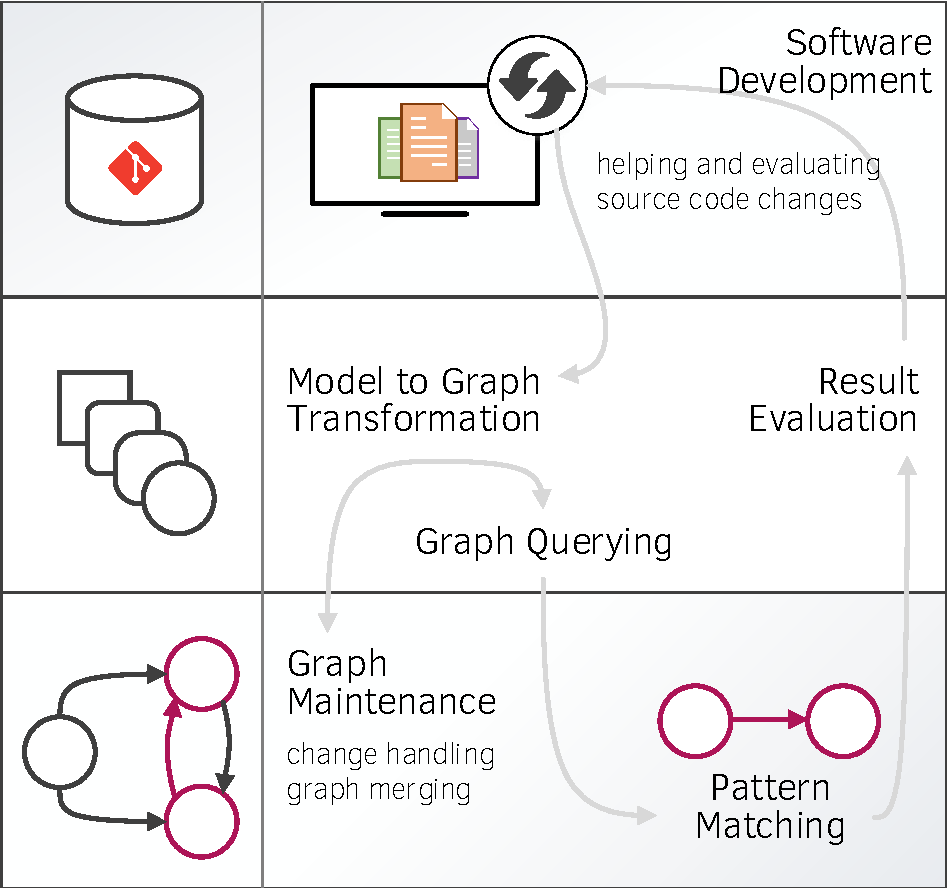
\includegraphics[width=\textwidth]{include/figures/architecture.pdf}
  \caption{Architecture Overview of the Approach}
  \label{fig:architecture-overview}
\end{figure}

\section{Main Components}

\section{Steps of Processing}

\chapter{Elaboration of the Workflow}
\label{chap:elaboration-of-the-workflow}

\chapter{Evaluation of the Prototype}
\label{chap:evaluation-of-the-prototype}

\chapter{Future Vision}
\label{chap:future-vision}

\chapter{Conclusions}
\label{chap:conclusions}


\backmatter{}
\pagenumbering{roman}
\setcounter{page}{\thesavepage}

\chapter*{Acknowledgments}
\addcontentsline{toc}{chapter}{Acknowledgments}
\label{chap:acknowledgments}
\thispagestyle{plain}

First, I would like to thank Dr. István Ráth and Zoltán Ujhelyi for providing the scientific foundations for my research and insight into software model verification.

I would like to thank my supervisors Ádám Lippai, Dávid Honfi, and Gábor Szárnyas for their friendly advice and enthusiasm. Also, I wish to express my gratitude to all other colleagues at Tresorit and the Fault Tolerant Systems Research Group who provided numerous valuable observations and suggestions.

Last but not least, I am deeply grateful to my family and friends for their continuous support.


%\section*{Awards}
%I am also thankful for the two awards supporting my work.
\vfill

\paragraph{Microsoft Azure for Research Award}
This report was supported by Microsoft Azure making it possible to use cloud resources with ease.

\paragraph{New National Excellence Program}
This report was supported by the ÚNKP-16-2-I. New National Excellence Program of the Ministry of Human Capacities.

\begin{center}

\includegraphics[width=0.3\textwidth]{include/figures/min_en.jpg}
\end{center}


\listoffigures*\addcontentsline{toc}{chapter}{List of Figures}
\listoftables*\addcontentsline{toc}{chapter}{List of Tables}

\printbibliography{}

\appendix
\chapter*{Appendix}\addcontentsline{toc}{chapter}{Appendix}


\label{page:last}

\end{document}
